The polyhedral framework was first used to examine the energy usage of
(and the execution time) of the Polybench programs and LULESH on the Intel Sandy Bridge
architecture. These programs are
written to allow easy framework manipulation of the program. 
A more realistic application \emph{brdr2d} on both the Intel Sandy Bridge
and the Intel Xeon Phi architectures is then studied.

\subsection{Execution Time and Energy Consumption Correlation}
The first experiments verify the relationship between execution time and energy consumption.

\subsubsection{Polybench}
The Polybench v3.2 contains 30 programs. Because of the large number of variants
created, the energy consumption of 2 (\emph{covariance} benchmark and \emph{2mm} benchmark)
were chosen for closer examination.
Figure~\ref{fig:TE} shows the relationship between the execution time and the 
energy usage for the 5135 variants of the \emph{covariance} benchmark, sorted by execution time.
The left y-axis shows the energy consumption (in joules) and the right y-axis shows the 
execution time (in seconds).

There is clear correlation between the time and the energy. The
energy line (blue, mostly the bottom) generally follows the time line.  
The best optimized program variant for time (bottom right in the figure)  
consumed the least amount of energy. The energy line has many places 
where 2 runs that take the same amount of time consume significantly different
energy. These appear as spikes in the graph. Examining the data,
we noticed that the higher energy usage value always had the ``maxfuse'' flag set.
The last jump is at variant 4236, above which all executions have ``maxfuse'' set.
The executable with ``maxfuse'' requires significantly more power than 
with either ``smartfuse'' or ``nofuse''.  For the executables where
no performance improvement is gained, this has noticeable energy costs.  However,
when the polyhedral framework finds the correct tiling size, the ``maxfuse''
flag produces a significantly fast executable (note the change in the
execution curve that occurs at variant 4236).
The ``smartfuse'' and ``no fuse'' options produce executables that run at lower power and may be beneficial if
peak power usage is a constraint, but longer execution times (up to $2\times$) result
in significantly higher overall energy costs.
The interaction between optimizations can have significant impact on
their effectiveness for both time, energy and power.

%The 
%observation is that while ``smartfuse/nofuse'' loop fusion maintained low usage of
%power (indicated by the constant gap between the two lines at the non-spike area),
% it did not achieve optimal even it was combined with all other possible transformations.
%For example, the figure shows that ``smartfuse/nofuse'' achieved close to optimal
%energy consumption (at about 550 joules before the last spike) but non-optimal 
%execution time (at 4.5 seconds before the last spike). On the other hand, while 
%``maxfuse'' program variants consumed energy at a higher rate (higher watts), it 
%had much better chance to get optimal execution time. For example, the program variants
%combining ``maxfuse'' and good tiling size ($32\times16\times1$) consumed the minimum amount of energy. 
%Other than that, the program variants after the last spike (starting from 4236) 
%all contain "maxfuse". 

%``Maxfuse'' and good tiling sizes
%are two major factors determining the execution time of \emph{covariance} program variants, which, by the 
%time/power/energy formula, determines the energy consumption. ``Maxfuse'' added with
%good tiling transformations can be optimal in both execution time and energy consumption, even though the power level is high. Similarly, bad tiling size and maxfuse can 
%lead to bad scenario where both the execution time 
%and the energy consumption are almost the worst case. The evidence can be obtained from 
%the graph where the energy line goes above the time line. For ``smartfuse'' and ``no fuse'',
%good tiling can lead to best power level, but probably not optimal energy consumption (not best execution).


\begin{figure}[bt]
    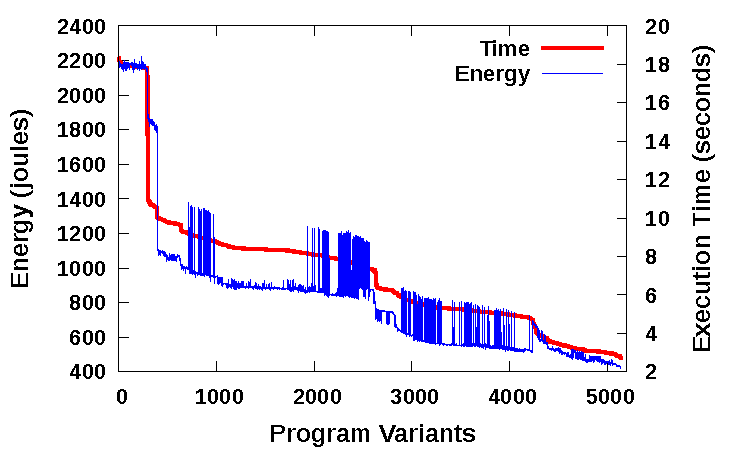
\includegraphics[width=3.5in]{Covariance}
%    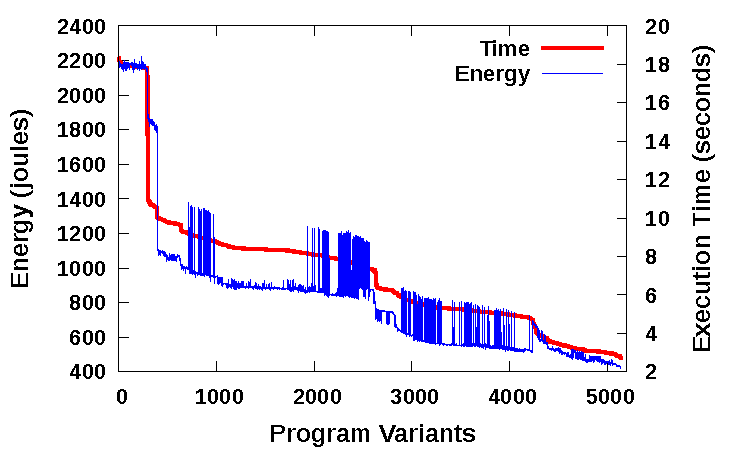
\includegraphics{Covariance}
    \caption{Graph showing the relationship between the execution time and the
energy consumption of all \emph{covariance} Polybench program variants on Sandy 
Bridge Processor (sorted by execution time). The spikes are caused by ``maxfuse''
loop transformation.}
    \label{fig:TE}
\end{figure}

\begin{figure}[bt]
    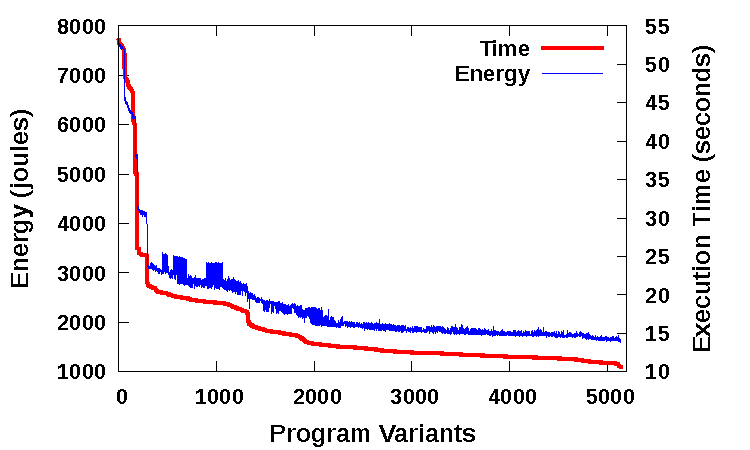
\includegraphics[width=3.5in]{2mm}
%    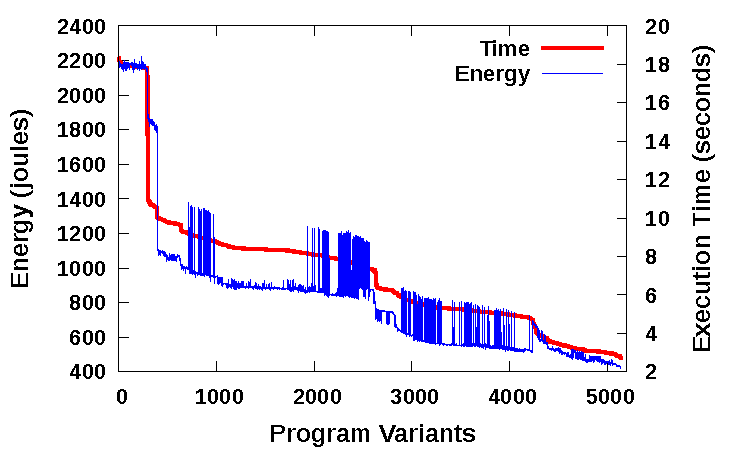
\includegraphics{Covariance}
    \caption{Graph showing the correlation between the execution time and the
energy consumption of \emph{2mm} Polybench on Sandy Bridge Processor (sorted by execution time).
The spikes are caused by bad tiling configuration.}
    \label{fig:2mm-TE}
\end{figure}

A similar correlation between execution time and energy occurs for the \emph{2mm} benchmark 
(as shown in Figure~\ref{fig:2mm-TE}). No single optimization has as great an effect on power
as ``maxfuse'' did in the previous example. The spikes that do occur (especially the left side)
are from poor tiling configurations. Power is approximately constant for all the runs, so energy
consumption is a function of execution time.

\subsubsection{Modified LULESH}

\begin{figure}[bt]
    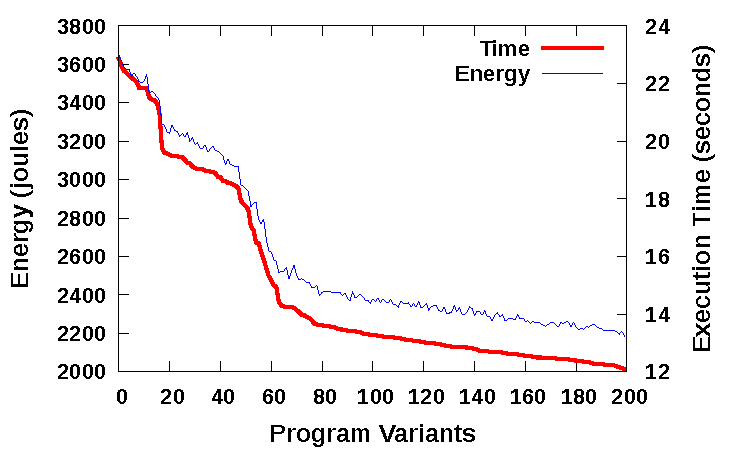
\includegraphics[width=3.5in]{lulesh-correlation}
    \caption{Graph showing the correlation between the execution time and the 
energy consumption of LULESH program on Sandy Bridge Processor (sorted by execution 
time).}    
    \label{fig:lulesh-correlation}
\end{figure}

For 200 variants of LULESH, Figure~\ref{fig:lulesh-correlation} shows the energy used and 
execution time. The energy curve mirrors the execution time. A slight ($<2\%$)
run-to-run variation in the energy, presents a minor
opportunity for energy tuning beyond execution time. LULESH optimizations 
overall provide almost a $2\times$ reduction in execution time 
(22.9 vs 12.1 seconds - 47\% reduction) and a significant decrease in energy (3650 vs 2185 Joules - 40\% reduction).
No optimizations resulted in a significant increase in power, although the power
required did rise slightly (from 160 Watts to 180 Watts - 12\% increase).

\subsubsection{Realistic Application}

\begin{figure*}[bt]
\centering
\subfigure[Time and energy correlation on Sandy Bridge] {
  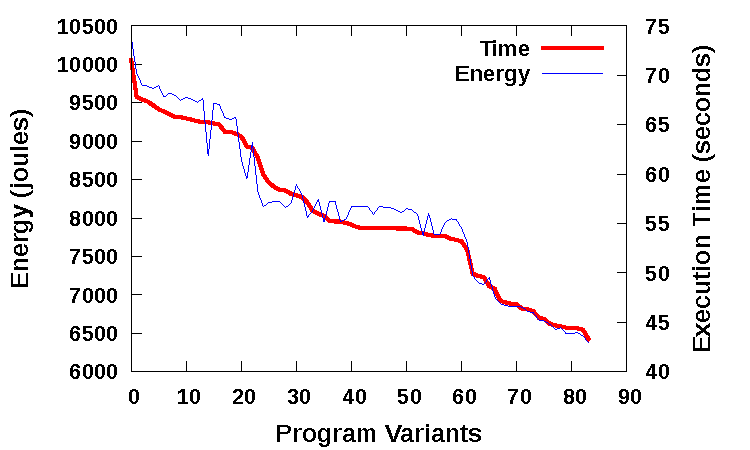
\includegraphics[width=0.45\textwidth]{Sandy-Brdr2d}
  \label{Sandy-correlation}
}
\subfigure[Time and energy correlation on MIC] {
  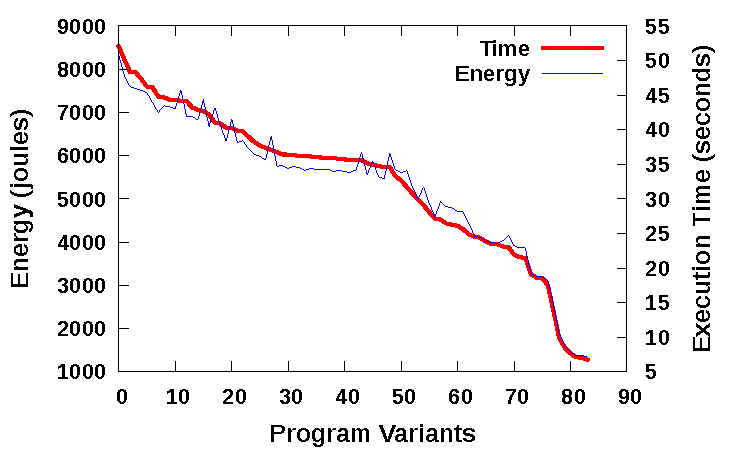
\includegraphics[width=0.45\textwidth]{MIC-Brdr2d}
  \label{MIC-correlation}
}
\caption{Graph showing the correlation between the execution time and the energy 
consumption of \emph{brdr2d} on Sandy Bridge processor and
on MIC architecture (both sorted by execution time).}
\label{fig:Brdr2d-TE}
\end{figure*}

\emph {brdr2d} contains two symmetric SCoPs (because of loop unswitching).
Each SCoP contained 42 statements. The number of dependencies between these 
statements was 638 (there were no loop carried dependencies). PolyOpt
detected and applied loop fusion (maxfuse or smartfuse) and loop tiling transformations
(various tile sizes) as
well as vectorization and auto-parallelization to the SCoPs. The fastest 84 program
variants were chosen for study on both the Sandy Bridge processor and Xeon Phi coprocessor.
49 of the 84 programs had ``maxfuse'' flag turned on.

Figure~\ref{fig:Brdr2d-TE} compares execution time and energy consumption  (for 2048 input size) for
the cardiac simulation application on the Sandy Bridge processor and on Xeon Phi card.
Both Figure~\ref{Sandy-correlation} and Figure~\ref{MIC-correlation} show that the
energy tracks the time. Saving energy consumptions is consistent with 
improving performance on both processors.
The energy line is above the time line for about half of Figure~\ref{Sandy-correlation}.
Those variants have ``smartfuse'' set, which in this case increases the power
required by the application (and therefore energy).
Figure~\ref{MIC-correlation} has the time line above
the energy line for the left half but below for the right half. 
For the Phi, the ``smartfuse'' option used lower power than ``maxfuse''.
The performance of ``maxfuse'' was much better than ``smartfuse''
and the overall execution time and energy use for ``maxfuse'' was lower (up to $5\times$).

\subsection{Polyhedral Optimization Results on the Realistic Application}
Optimizing \emph{brdr2d} on the Sandy Bridge Processor and on Phi coprocessor show the
advantage using the polyhedral framework to optimize for
both execution time and energy.

\subsubsection{Results on Sandy Bridge Processor}

To better understand the optimization variants of \emph {brdr2d}
they were executed with four different input sizes. Figure~\ref{fig:speedup}
compares the best variant for each input size
with the base-line OpenMP version. The optimal tiling was different as the
input grew. For the 256 case $1\times128$ resulted in the fastest
execution, For the larger cases, the variant with tile size $1\times256$ was 
fastest. As the problem size grew the optimized variants' relative performance and
energy consumption improved (256 - $2.5\%$ to 2048 - $21\%$). As the loop size
increases and the loop nest becomes a more dominant portion of the execution,
the relative performance from optimization improves.
For the smaller sizes the data fit into various cache levels and the 
benefits of loop optimizations for data locality are ineffective.

\begin{figure}[bt]
    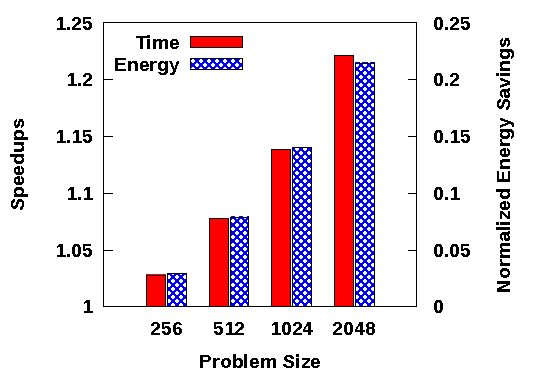
\includegraphics[width=3.2in]{speedup}
    \caption{Graph showing the performance improvement and energy savings of 
the optimal program variant over the baseline OpenMP implementation for 
different problem size on Sandy Bridge Processor.} 
    \label{fig:speedup}
\end{figure}

\subsubsection{Results on Intel Xeon Phi}
To show the benefits of using polyhedral optimization techniques on the Phi
accelerator card, the performance of a manual OpenMP implementation 
can be compared with the best Polyopt/PoCC generated OpenMP program variant (shown in Figure~\ref{fig:MIC-speedup-over-seq}).
The speedups were calculated against a sequential Sandy Bridge execution.

The best PoCC variant of \emph{brdr2d}, is over $20\%$ faster than the baseline Phi version for small sizes.
For the largest size, 2048, the best Polyopt/PoCC variant is still slightly better than the
baseline and has an absolute speed up of over $150\times$.
The optimal tiling size changes as the input grows. In each case, $1\times size$
is preferred for maximum vectorization. As the problem size grows, non-tiled
vectorization improves, reducing the effectiveness of tiling.
As expected the two main performance drivers for the Phi are 
parallelization, for threads, and vectorization, within threads.

The polyhedral optimizations also improves energy. Figure~\ref{fig:MIC-speedup} shows the \emph{relative} speedups and the
normalized energy savings offered by the polyhedral transformations and auto-parallelization.
The energy savings approximately match the relative speedups, ranging from $20\%$
down to $3\%$ as size increases (and baseline vectorization improves).
\begin{figure}[bt]
    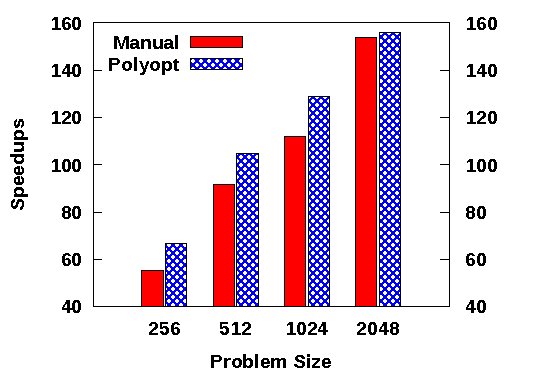
\includegraphics[width=3.2in]{Speedup-over-sequential}
    \caption{Graph showing the comparison between speedups of manual OpenMP implementation and the best
Polyopt/PoCC generated OpenMP program variant over the sequential implementation on MIC architecture.}
    \label{fig:MIC-speedup-over-seq}
\end{figure}
\begin{figure}[bt]
    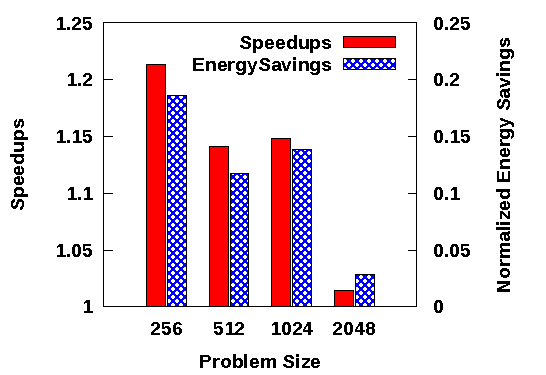
\includegraphics[width=3.2in]{MIC-Speedups}
    \caption{Graph showing the performance improvement and energy savings of 
the optimal Polyopt/PoCC generated program variant over the baseline OpenMP implementation for different problem size on
MIC architecture.}
    \label{fig:MIC-speedup}
\end{figure}
